\chapter{Replace with Title}
\label{ch:chapter2}

Please remove all sample text, including figures and tables, and replace it
with your work. Below are some examples of figures, tables, equations, and
citations.

\section{Figure Example}

All figures and tables in your work must be properly referenced in the text.
For example, below you will find a picture of the Nittany Lion
(Fig.~\ref{fig:nittany-lion}). All figure captions go directly beneath the
figure.

\begin{figure}[htbp]
  \centering
  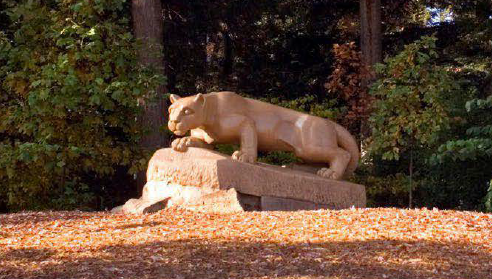
\includegraphics[width=0.6\textwidth]{nittany-lion}
  \caption{The Nittany Lion}
  \label{fig:nittany-lion}
\end{figure}

\section{Table Example}

All table captions go directly above the table. Please see the example
(Table~\ref{tab:front-matter}) below.

\begin{table}[htbp]
  \centering
  \caption{Front Matter Requirements}
  \label{tab:front-matter}
  \setlength{\tabcolsep}{5pt}
  \begin{tabular}{lll}
    \toprule
    \tableheading{Page} & \tableheading{Required} & \tableheading{Visible Page Number} \\
    \midrule
    Title Page & Mandatory & No \\
    Committee Page & Mandatory & Yes \\
    Abstract & Mandatory & Yes \\
    Table of Contents & Mandatory & Yes \\
    List of Figures & Mandatory (if figures used) & Yes \\
    List of Tables & Mandatory (if tables used) & Yes \\
    Acknowledgments & Mandatory (if federal funding used) & Yes \\
    Frontispiece & Optional & Yes \\
    List of Symbols/List of Abbreviations & Optional & Yes \\
    Dedication & Optional & Yes \\
    \bottomrule
  \end{tabular}
\end{table}

\section{Equation Example}

Number equations that you refer to, and reference them with
\verb|\eqref|, e.g., Equation~\eqref{eq:example}:
\begin{equation}
  \label{eq:example}
  e^{i\pi} + 1 = 0.
\end{equation}

\section{Citation Example}

Add BibTeX entries to \texttt{references.bib} and cite them with
\verb|\cite|, e.g., \cite{lamport1994latex,knuth1984texbook}. The reference
list is generated automatically.
